\chapter{Datasets} \label{sec:appendix_datasets}

\section{Tabular datasets} \label{sec:tabular_datasets}
In total, we have collected $40$ tabular datasets, the majority of which come from the UCI repository~\cite{Dua:2019}. The complete listing of dataset dimensions is recorded in Tab.~\ref{tab:tabular_datasets_anomaly} and~\ref{tab:tabular_datasets_classification}. Except for the ANNThyroid, Arrhytmia, HAR, HTRU2, KDD Cup 99 (small), Spambase, Mammography, and Seismic, where the anomaly class has a clear meaning (security incident or disease), we have followed the technique of~\cite{emmott2013systematic} for creating artificial datasets for anomaly detection tasks from classification datasets. More precisely, we have used only "easy" and "medium" anomalies, as "hard" and "very hard" are not truly anomalous in the sense of being statistically distinct from the normal class.

\begin{table}
    \centering
    \tabcolsep=0.1cm
    \begin{tabular}{llrrr}
    \toprule
    \textbf{dataset} & \textbf{alias} & \textbf{dim} & \textbf{anom} & \textbf{normal}   \\\midrule
    ANNthyroid & ann  & 21 & 534 & 6665 \\
    Arrhythmia & arr  & 275 & 206 & 245 \\
    HAR & har & 561 & 1944 & 8355  \\
    HTRU2 & htr & 8 & 1638 & 16257  \\
    KDD99 (10\%) & kdd & 118 & 396742 & 97276  \\
    Mammography & mam & 6 & 260 & 10921  \\
    Seismic & sei  & 24 & 170 & 2412  \\
    Spambase & spm & 57 & 1812 & 2786  \\
    \\\bottomrule
    \end{tabular}
    \vspace*{0.15cm}
    \caption{Basic statistics (dimensionality, number of normal and anomalous samples) of the tabular dataset designed directly for anomaly detection.}
    \label{tab:tabular_datasets_anomaly}
\end{table}

\begin{table}
    \centering
    \tabcolsep=0.1cm
    \begin{tabular}{llrrr}
    \toprule
    \textbf{dataset} & \textbf{alias} & \textbf{dim} & \textbf{anom} & \textbf{normal}   \\\midrule
    Abalone & aba & 10 & 50 & 2151  \\
    Blood Transfusion & blt & 4 & 16 & 382  \\
    Breast Cancer Wisconsin & bcw  & 30 & 206 & 356 \\
    Breast Tissue & bts & 9 & 22 & 65 \\
    Cardiotocography & crd & 27 & 228 & 1830  \\
    Ecoli & eco & 7 & 108 & 205  \\
    Glass & gls & 10 & 94 & 112  \\
    Haberman & hab & 3 & 14 & 225  \\
    Ionosphere & ion & 33 & 122 & 225  \\
    Iris & irs & 4 & 46 & 100  \\
    Isolet & iso & 617 & 3300 & 4496  \\
    Letter Recognition & ltr & 617 & 3600 & 4196  \\
    Libras & lbr & 90 & 142 & 215  \\
    Magic Telescope & mgc & 10 & 3882 & 12331  \\
    Miniboone & mnb & 50 & 23922 & 93565  \\
    Multiple Features & mlt & 649 & 800 & 1200  \\
    PageBlocks & pgb & 10 & 384 & 4911  \\
    Parkinsons & prk & 22 & 44 & 146  \\
    Pendigits & pen & 16 & 5384 & 5537  \\
    Pima Indians & pim & 8 & 176 & 500  \\
    Sonar & snr & 60 & 96 & 110  \\
    Spect Heart & sph & 44 & 52 & 211  \\
    Statlog Satimage & sat & 36 & 2630 & 3592  \\
    Statlog Segment & seg & 18 & 938 & 1320  \\
    Statlog Shuttle & sht & 8 & 28 & 57767  \\
    Statlog Vehicle & vhc & 18 & 132 & 627  \\
    Synthetic Control Chart & scc & 60 & 200 & 400  \\
    Wall Following Robot & wrb & 24 & 2220 & 2921  \\
    Waveform-1 & wf1 & 21 & 1482 & 3302  \\
    Waveform-2 & wf2 & 21 & 1472 & 3302  \\
    Wine & wne & 13 & 70 & 106  \\
    Yeast & yst & 8 & 390 & 751   \\\bottomrule
    \end{tabular}
    \vspace*{0.15cm}
    \caption{Basic statistics of the tabular multi-class datasets that were transformed into anomaly detection problems.}
    \label{tab:tabular_datasets_classification}
\end{table}

\section{Image datasets} \label{sec:image_datasets}
The number of image datasets used for the evaluation of deep models is limited, as there are very few publicly available image datasets designed purely for anomaly detection. In our experiments, we have used the MNIST-C and MVTec-AD datasets. Furthermore, we have extended these with artificially created anomaly datasets based on common image datasets that are usually used for classification. These contain ten classes of distinct objects. In most of our experiments, we have used the leave-one-in protocol, where one of the classes is considered normal and the remaining are anomalous. Therefore, one classification image dataset with ten distinct classes is transformed into ten different anomaly detection sub-datasets. Finally, for the experiments with the SGVAEGAN model, we have created two completely artificial image datasets where the goal was to have images with prominent objects on a more or less unified background. Again, the basic statistics on image datasets are shown in Tab.~\ref{tab:image_datasets}.

\begin{description}

    \item[\textbf{MNIST}] dataset~\cite{lecun2010mnist} is a collection of greyscale images of handwritten digits and one of the most ubiquitous datasets used in machine learning due to its simplicity and easy interpretation.
    
    \item[\textbf{FashionMNIST}]~\cite{xiao2017fashion} is a classification dataset of low-resolution greyscale images of ten different classes of fashion articles, such as coats, shirts, or sandals. It is supposed to be slightly more difficult than the MNIST datasets.

    \item[\textbf{SVHN2}] is a well-known benchmark dataset~\cite{netzer2011reading} containing images of house numbers. In this cropped version of the dataset, the target digit is centered in the middle of the picture. However, there may be partial digits adjacent to it, which makes the problem harder. Furthermore, there are no available annotations for the background/foreground factor and in this paper, it is included mainly as a benchmark for comparison to other baseline methods. 
    
    \item[\textbf{CIFAR10}] is another classical dataset of images of 10 classes of different objects or animals often used for validation of anomaly detectors~\cite{ruff2018deep, ruff2019deep, chalapathy2018anomaly}. For an overview of the dataset see~\cite{krizhevsky2009learning}. 

    \item[\textbf{MNIST-C}] is an artificially created anomaly detection dataset introduced in~\cite{muMNISTCRobustnessBenchmark2019}. It is created using digits from the MNIST datasets to which certain distortions and corruptions are added. The normal data in this case are the original MNIST images and the anomalies are their corrupted counterparts. There are 15 classes of corruptions, such as different types of blur, noise, or geometrical transformations. The difficulty of the detection of corrupted images varies a lot. While brightness change is usually very easy for most detectors, translation or rotation is sometimes very difficult, see the extended results in the Appendix of~\cite{vskvara2021comparison}.

    \item[\textbf{MVTec-AD}] is an industrial dataset~\cite{bergmann2019mvtec} that captures several different problems of identifying faulty or damaged objects. We have included only some classes of the dataset that either represented an anomaly detection problem of a varying degree of difficulty or contained a prominent object in the foreground. The individual problems are smaller --- on average about 200 normal and 100 anomalous samples. The images used in our experiments are downscaled to 128x128 pixels from the original size of 1024x1024.
    
    \item[\textbf{Wildlife MNIST}]~\cite{sauer2021counterfactual} is an artificial dataset based on the standard MNIST. For each MNIST digit, a background and foreground texture is sampled from a texture dataset described in~\cite{cimpoi2014describing} to create a colored version. Two versions of this dataset were created - \textit{mixed} and \textit{non-mixed}. In the mixed version, the background and foreground for each digit are sampled randomly from 10 background and foreground texture classes to create a very diverse set of images. In the non-mixed version, the background and foreground class is kept the same for all basic MNIST digits from the same class, resulting in a less diverse dataset. For examples of the non-mixed version, see the top row of Fig.~\ref{fig:wmnist_grid}. Each version contains 60000 samples of RGB images with three factors of variation.
    
    \item[\textbf{COCOPlaces}] is a dataset created similarly to Wildlife MNIST. 10 classes of objects from the COCO dataset~\cite{lin2014microsoft} were combined with 10 background classes from the Places dataset~\cite{zhou2017places}. Again, mixed and non-mixed variants were created. Because the object shape and texture cannot be separated in this case, it represents a problem with two factors of variation that is slightly more realistic than the previous one. Furthermore, it is much harder, as the object shapes are very distinct, sometimes the foreground object is only partially visible and the background itself may sometimes contain some other objects as well. A total of 5000 RGB images were generated for each variant. For sample images of all classes, see~Fig.~\ref{fig:all_grid}.
    % the object classes are 'boat', 'airplane', 'truck','dog','zebra','horse','bird','train','bus','motorcycle'
    % the background classes are 'beach', 'bamboo_forest','canyon','broadleaf forest','ball_pit','orchard','rock_arch','shower','ski_slope','wheat_field'
\end{description}

\begin{table}
    \centering
    \tabcolsep=0.1cm
    \begin{tabular}{lllrr}
    \toprule
    \textbf{dataset} & \textbf{alias} & \textbf{dim} & \textbf{anom} & \textbf{normal} \\
    \midrule
    MNIST-C & mnistc & 28x28x1 & 70000 & 70000 \\
    MVTec-AD - wood & wood & 128x128x3 & 60 & 266 \\
    MVTec-AD - grid & grid & 128x128x3 & 57 & 285 \\
    MVTec-AD - transistor & transistor & 128x128x3 & 40 & 273 \\
    MVTec-AD - bottle & transistor & 128x128x3 & 40 & 273 \\
    MVTec-AD - capsule & transistor & 128x128x3 & 40 & 273 \\
    MVTec-AD - nut & transistor & 128x128x3 & 40 & 273 \\
    MVTec-AD - pill & transistor & 128x128x3 & 40 & 273 \\
    FashionMNIST & fmnist & 28x28x1 & 63000 & 7000   \\
    MNIST & mnist & 28x28x1 & 63686 & 6312  \\
    CIFAR10 & cifar10 & 32x32x3 & 54000 & 6000  \\
    SVHN2 & svhn2 & 32x32x3 & 80327 & 18960  \\
    Wildlife MNIST & wmnist & 32x32x3 & 54000 & 6000  \\
    COCOPlaces & coco & 64x64x3 & 4500 & 500  \\\bottomrule
    \end{tabular}
    \vspace*{0.15cm}
    \caption{Basic statistics of image datasets. Note that the numbers of normal and anomalous samples are approximate, as each dataset (apart from MVTec-AD) has 10 classes of data and some datasets have an uneven distribution of the number of samples in these classes.}
    \label{tab:image_datasets}
\end{table}
    

% what is missing - mnist, mnistc, fashionmnist
\begin{figure}
    \centering
    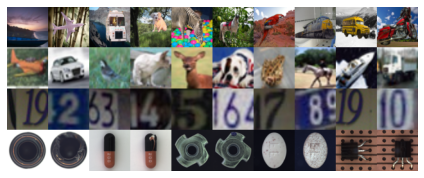
\includegraphics[width=\textwidth]{data/chapter_sgvaegan/fig5_all_grid.png}
    \caption{Samples from the semantic image datasets and the MvTec-AD dataset which were used in the experiments. Datasets from the top row to bottom: COCOPlaces, CIFAR10, SVHN2, and MVTec-AD. MVTec-AD examples of normal and anomalous samples from the \textit{bottle, capsule, metal nut, pill}, and \textit{transistor} classes are shown.}
    \label{fig:all_grid}
\end{figure}
